%%%%%%%%%%%%%%%%%%%%%%%%%%%%%%%%%%%%%%%%%
% Short Sectioned Assignment LaTeX Template Version 1.0 (5/5/12)
% This template has been downloaded from: http://www.LaTeXTemplates.com
% Original author:  Frits Wenneker (http://www.howtotex.com)
% License: CC BY-NC-SA 3.0 (http://creativecommons.org/licenses/by-nc-sa/3.0/)
%%%%%%%%%%%%%%%%%%%%%%%%%%%%%%%%%%%%%%%%%

%----------------------------------------------------------------------------------------
%	PACKAGES AND OTHER DOCUMENT CONFIGURATIONS
%----------------------------------------------------------------------------------------

\documentclass[paper=a4, fontsize=11pt]{scrartcl} % A4 paper and 11pt font size

% ---- Entrada y salida de texto -----

\usepackage[T1]{fontenc} % Use 8-bit encoding that has 256 glyphs
\usepackage[utf8]{inputenc}
%\usepackage{fourier} % Use the Adobe Utopia font for the document - comment this line to return to the LaTeX default

% ---- Idioma --------

\usepackage[spanish, es-tabla]{babel} % Selecciona el español para palabras introducidas automáticamente, p.ej. "septiembre" en la fecha y especifica que se use la palabra Tabla en vez de Cuadro

% ---- Otros paquetes ----

\usepackage{url} % ,href} %para incluir URLs e hipervínculos dentro del texto (aunque hay que instalar href)
\usepackage{amsmath,amsfonts,amsthm} % Math packages
%\usepackage{graphics,graphicx, floatrow} %para incluir imágenes y notas en las imágenes
\usepackage{graphics,graphicx, float} %para incluir imágenes y colocarlas
\usepackage{listings}
\usepackage{subfig}

% Para hacer tablas comlejas
%\usepackage{multirow}
%\usepackage{threeparttable}

%\usepackage{sectsty} % Allows customizing section commands
%\allsectionsfont{\centering \normalfont\scshape} % Make all sections centered, the default font and small caps

\usepackage{fancyhdr} % Custom headers and footers
\pagestyle{fancyplain} % Makes all pages in the document conform to the custom headers and footers
\usepackage{eurosym} % Para poder añadir el símbolo del euro
\fancyhead{} % No page header - if you want one, create it in the same way as the footers below
\fancyfoot[L]{} % Empty left footer
\fancyfoot[C]{} % Empty center footer
\fancyfoot[R]{\thepage} % Page numbering for right footer
\renewcommand{\headrulewidth}{0pt} % Remove header underlines
\renewcommand{\footrulewidth}{0pt} % Remove footer underlines
\setlength{\headheight}{13.6pt} % Customize the height of the header

\numberwithin{equation}{section} % Number equations within sections (i.e. 1.1, 1.2, 2.1, 2.2 instead of 1, 2, 3, 4)
%\numberwithin{figure}{section} % Number figures within sections (i.e. 1.1, 1.2, 2.1, 2.2 instead of 1, 2, 3, 4)
%\numberwithin{table}{section} % Number tables within sections (i.e. 1.1, 1.2, 2.1, 2.2 instead of 1, 2, 3, 4)

\setlength\parindent{0pt} % Removes all indentation from paragraphs - comment this line for an assignment with lots of text

\newcommand{\horrule}[1]{\rule{\linewidth}{#1}} % Create horizontal rule command with 1 argument of height

% Margins
\usepackage[margin=1.25in]{geometry}

% Begin section numbering at 0
\setcounter{section}{-1} 

% Hyperlinks
\usepackage{hyperref, xcolor}
\hypersetup{
  % hidelinks = true,   % Oculta todos los enlaces.
  colorlinks = true,   % Muestra todos los enlaces, sin bordes alrededor.
  linkcolor={black},     % Color de enlaces genéricos
  citecolor={black!40!blue},   % Color de enlaces de referencias
  urlcolor={black!40!blue}     % Color de enlaces de URL
}
  % Configuración del documento

%----------------------------------------------------------------------------------------
%	TÍTULO Y DATOS DE LOS ALUMNOS
%----------------------------------------------------------------------------------------

\title{	
	\normalfont \normalsize 
	\textsc{\textbf{Recuperación de Información (2019-2020)} \\ Doble grado en Informática y Matemáticas \\ Universidad de Granada} \\ [25pt] 
	\horrule{0.5pt} \\[0.4cm]
	\huge Práctica 1: Parser de Documentos con TIKA  \\ 
	\horrule{2pt} \\[0.5cm] 
}

\author{Simón López Vico \\ Miguel Cantarero López \\ Alberto Jesús Durán López} 
\date{\normalsize\today}

%----------------------------------------------------------------------------------------
% DOCUMENTO
%----------------------------------------------------------------------------------------

\begin{document}
\maketitle       % título
\newpage 
\tableofcontents % índice
\newpage

\section{Introducción}
En esta práctica veremos cómo extraer información con Tika a partir de un documento dado, independientemente del formato del archivo, paso previo para cualquier proceso de recuperación de información o análisis de textos.
	
Hemos realizado un programa capaz de extraer información de los archivos que cuelgan de un directorio, pasado como entrada al programa. Las diferentes opciones son:

\section{Opción -d}
\begin{itemize}
		\item -d : Se muestra una tabla que contiene el nombre del fichero, tipo, codificación e idioma. 
		
		Primero de todo, tomamos el archivo y usando la función \textit{parse} de tika, parseamos dicho archivo junto a \textit{metada}, variable de tipo \textit{Metadata}, declarada al principio del programa y común para todas las opciones.
		
		A continuación, detectamos el MIME del archivo, extraemos el texto plano en un string y por último, el idioma, la codificación y el nombre.
\end{itemize}
\lstset{language=C, breaklines=true, basicstyle=\footnotesize}
\begin{lstlisting}[frame=single]
//Se parsean los ficheros pasados como argumento y se extrae el contenido
for(String f : ficheros){
	File file = new File("./"+args[0]+"/"+f);
						
	//Parseamos
	tika.parse(file, metadata);
	String contenido = tika.parseToString(file);            
	
	// Detectamos el MIME tipo del fichero
	String type = tika.detect(file);
	
	//Extraemos el texto plano en un string
	String text = tika.parseToString(file);
	
	//Extraemos el idioma
	String idioma = identifyLanguage(contenido);
	
	//Extraemos la codificacion y el nombre
	String cod = metadata.get(Metadata.CONTENT_ENCODING);
	String name = metadata.get(Metadata.RESOURCE_NAME_KEY);
}
\end{lstlisting}

\newpage
\section{Opción -l}
\begin{itemize}
	\item -l : Se obtienen todos los enlaces extraíbles de cada documento. 
	
	Primero, una vez abierto el archivo a extraer los links, declaramos todas las variables (de tipo \textit{LinkContentHandler, ContentHandler, TeeContentHandler y ParseContext}) necesarias para dicha opción. 
	
	A continuación, detectamos el fichero , proceso previo a parsear.
	Como para la función \textit{parser} necesitamos una variable de tipo \textit{InputStream}, la declaramos a partir de nuestro fichero \textit{file} y parseamos. \\
	Por último, extraemos los links de la variable \textit{linkHandler} y los mostramos por pantalla.
\end{itemize}
	
\lstset{language=C, breaklines=true, basicstyle=\footnotesize}
\begin{lstlisting}[frame=single]
for(String f : ficheros){
	File file = new File("./"+args[0]+"/"+f);
	
	//Declaracion de variables necesarias para extraer los links
	LinkContentHandler linkHandler = new LinkContentHandler();
	ContentHandler textHandler = new BodyContentHandler();
	TeeContentHandler teeHandler = new TeeContentHandler(linkHandler);
	ParseContext parseContext = new ParseContext();
	
	//Creamos variable de tipo InputStream a partir del fichero 'file'
	InputStream target = new FileInputStream(file);

	//Detectamos el fichero. Proceso previo a parsear
	AutoDetectParser parser = new AutoDetectParser();

	//Parseamos 
	parser.parse(target,teeHandler,metadata,parseContext);
					
	List<Link> links=linkHandler.getLinks();
	System.out.println("LINKS EN EL ARCHIVO " +file.getName()+ ":");
					
	if(links.isEmpty())
		System.out.println("No hay links :(");
	else
		for(Link link:links)
	System.out.println(link);					
}
\end{lstlisting}

\newpage	
	
\section{Opción -t}
\begin{itemize}
	\item -t : Para cada documento se genera un fichero con formato CSV en el que se muestra cada palabra junto a su ocurrencia.
	
	Comenzaremos extrayendo el texto plano del documento por completo, al cuál aplicaremos la función \texttt{split([...])} usando una expresión regular, que creará un vector con todas las palabras del texto. La expresión regular se encargará de reconocer como palabras los elementos del texto plano que estén separados por:
	\begin{itemize}
	\item Uno o más espacios.
	\item Uno o dos puntos, una coma o un punto y coma seguidos de uno más espacios.
	\item Paréntesis, interrogaciones, exclamaciones, etc.
	\end{itemize}
	
	Una vez obtenidas todas las palabras, recorremos el vector creado para contar el número de ocurrencias de cada una de ellas; tras ello, eliminaremos los caracteres erróneos contados\footnote{A veces se guardan palabras vacías.}.
	
	Finalmente, ordenaremos las palabras por su número de ocurrencias de mayor a menor y las añadiremos a un fichero CSV.
\end{itemize}

\lstset{language=C, breaklines=true, basicstyle=\footnotesize}
\begin{lstlisting}[frame=single]
for(String f : ficheros){
	File file = new File("./"+args[0]+"/"+f);
   					
	// Parseamos el fichero y obtenemos su texto plano.
   	tika.parse(file, metadata);
   	String contenido = tika.parseToString(file);
   					
   	// Separamos todas las palabras que aparecen en el fichero y las anadimos a vector
   	String[] todas=contenido.split("\\s+|[\\.\\;\\:\\,]\\s+|[()?!]");
   					
   	// Creamos un ArrayList donde guardaremos el numero de veces que se repite cada palabra
   	ArrayList<PalabraOcurrencias> palaocu=new ArrayList<PalabraOcurrencias>();
   	
	//Recorremos todas las palabras. Si la palabra ya se encuentra aumentamos el contador
	//de dicha palabra. En casa contraria la introducimos en 'palaocu'
   	for(String palabra:todas){
   		Boolean encontrado=false;
   		int i=0;				
   		while(i<palaocu.size() && !encontrado){
   			if(palaocu.get(i).palabra.compareTo(palabra)==0)
   				encontrado=true;
   			else
   				i++;
   		}					
   		if(encontrado)
   			palaocu.get(i).ocurrencias++;
   		else
   			palaocu.add(new PalabraOcurrencias(palabra, 1));
   	}			

	// Eliminamos las palabras que no queremos tratar
	String filename="./CSV";
	if(rminutiles){
		[...]
		filename+="/rminutiles/"+file.getName()+"_inutiles.csv";
	}else{
		[...]
		filename+="/normal/"+file.getName()+".csv";
	}
					
	// Ordenamos las palabras con su numero de ocurrencias en orden descendente
	Collections.sort(palaocu, new SortbyOcurrencias());
	
	// Anyadimos la informacion al fichero CSV
	String palcsv="";
	
	for(int i=0; i<palaocu.size(); i++){
		palcsv+=palaocu.get(i).palabra+";"+palaocu.get(i).ocurrencias+"\n";
	}
	
	PrintWriter writer = new PrintWriter(filename);
	writer.print(palcsv);
	writer.close();
}
\end{lstlisting}
\vspace{0.3cm}

El resultado obtenido tras ejecutar este código sobre el poema de Homero \textit{"La Odisea"} es el siguiente:

\begin{lstlisting}[frame=single]
	de;8120
	y;7112
	a;6959
	que;5599
	la;5043
	[...]
	Ulises;1674
	por;1452
	[...]
	Telemaco;734
	[...]
\end{lstlisting}
\vspace{0.3cm}

Podemos ver que las palabras más repetidas no aportan información importante sobre el texto, por lo que desarrollamos la siguiente opción.

\newpage

\section{Opción -t -rminutiles}
Esta opción permite mejorar la nube de palabras que podemos crear a partir del CSV que se obtiene de cada archivo. Actúa de la misma manera que la opción \texttt{-t}, pero elimina palabras que no aportan información del tema sobre el que trata el texto (determinantes,artículos, etc). Dichas palabras se extraerán del vector de ocurrencias de cada palabra en el mismo momento que eliminamos caracteres erróneos (visto en la anterior sección).

Al ejecutar esta nueva opción sobre \textit{"La Odisea"} obtenemos:
\begin{lstlisting}[frame=single]
	Ulises;1674
	Telemaco;734
	pretendientes;497
	Jupiter;478
	pues;464
	<<;436
	todos;403
	palacio;396
	[...]
\end{lstlisting}

\section{Nube de palabras}
Éstas son las dos nubes de palabras obtenidas tras generar los ficheros CSV del texto \textit{"La Odisea"} e introducir el documento CSV en la web \texttt{https://wordart.com/create}:

\begin{figure}[H]
\centering
\subfloat[Nube de palabras con la opción \texttt{-t} (izquierda) y \texttt{-t -rminutiles} (derecha).]{
		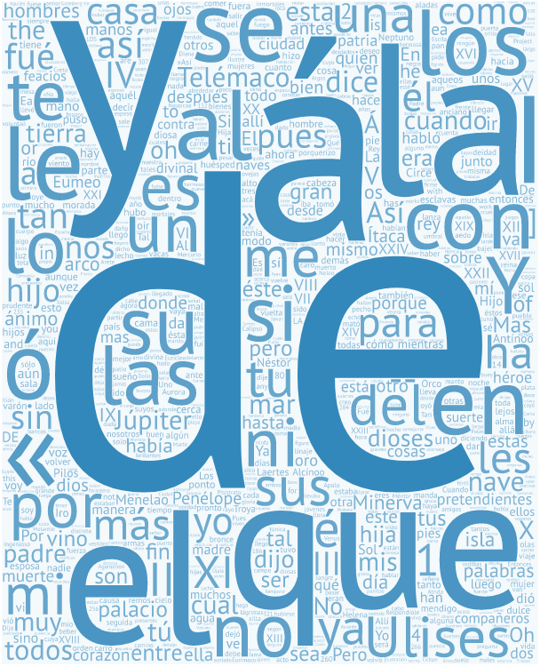
\includegraphics[scale=0.35]{images/nube.png}
		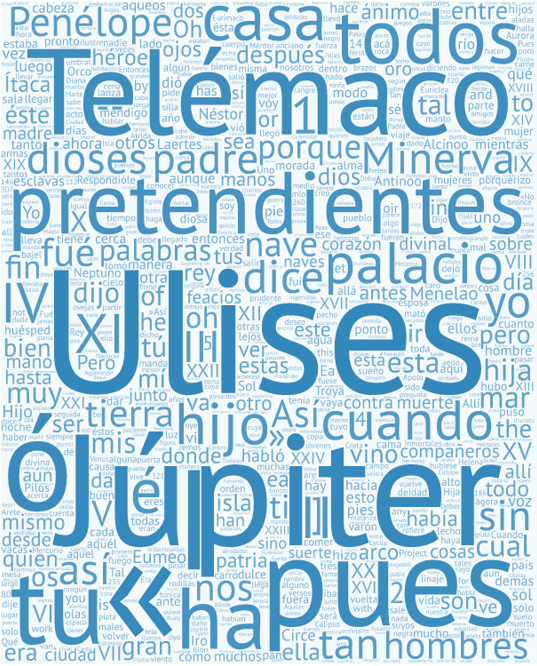
\includegraphics[scale=0.35]{images/nube_rminutiles.png}	
}
\end{figure}

\section{Compilación}
Situados en la carpeta \textit{code}, compilamos con el comando: \\
\textbf{javac -cp ../tika-app-1.22.jar p1.java PalabraOcurrencias.java} \\
y ejecutamos con \textbf{java -cp ../tika-app-1.22.jar:. p1 documentos -\textit{opción}}

\newpage
% -----------------------------------------------
% Bibliografía.
% -----------------------------------------------
\begin{thebibliography}{9}
	\bibitem{https://tika.apache.org/}
	\href{}{https://tika.apache.org/}
\end{thebibliography}

\end{document}